\documentclass[hidelinks, 10pt, pdf, hyperref={unicode}]{beamer}
\usepackage[czech]{babel}
\usepackage{graphics}
\usepackage{hyperref}
\usepackage[czech, linesnumbered, noline, longend, ruled]{algorithm2e}
\usepackage{times}
\setbeamertemplate{blocks}[rounded, shadow=true]
\usepackage{hyperref}

%\usetheme{CambridgeUS}        %Vzhled jednotlivych slidu
\usecolortheme{seahorse}    %Bareva slidu
\logo{\scalebox{0.22}{
\includegraphics{images/VUT.eps}}}    %Pridani loga do prezentaci
\setbeamertemplate{footline}[frame number]      %Pridani cislovani jednotlivych slidu
\author{Roman Machala (xmacha86)}   %autor, ten je v preambuli, protoze v begin{document} to hazelo chybu
%stejne tak zbytek je v begin{document} protoze v preambuli to hazelo chybu
%fix : https://tex.stackexchange.com/questions/10555/hyperref-warning-token-not-allowed-in-a-pdf-string

\begin{document}

%Titulni strana
\title{Typografie a publikování\,--\,5.projekt}
\subtitle{Kruskalův algoritmus}
\institute{
        Vysoké učení technické v Brně \\
        Fakulta informačních technologií
}   %instituce
\date{\today}
    
    \frame{\titlepage}
    \begin{frame}
        \frametitle{Obsah prezentace}
        \begin{itemize}
            \item{Myšlenka Kruskalova algoritmu} 
            \item{Minimální kostra grafu}
            \item{Princip Kruskalova algoritmu} 
            \item{Příklad Kruskalova algoritmu} 
            \item{Obecný postup Kruskalova algoritmu}
            \item{Použité zdroje}
        \end{itemize}
    \end{frame}

    \begin{frame}
        \frametitle{Myšlenka Kruskalova algoritmu}
        \begin{itemize}
            \item{Slouží k nalezení minimální kostry grafu (kostry takové, že součet vah jejich hran je minimální)}
            \item{Hrany grafu musejí mít nezáporné ohodnocení (délku)}
            \item{Všechny vrcholy původního grafu jsou i vrcholy minimální kostry}
        \end{itemize}
        \begin{block}{Algebraický zápis}
            $G(V,H)$, kde:
            \begin{itemize}
                \item{$G$ je graf}
                \item{$V$ je neprázdná množina vrcholů grafu $G$}
                \item{$H$ je neprázdná množina kladně ohodnocených hran grafu $G$}
            \end{itemize}
        \end{block}
    \end{frame}

    \begin{frame}
        \frametitle{Minimální kostra grafu}
        \begin{block}{Definice}
            Podgraf $T \subseteq G$ souvislého grafu $G$ se nazývá kostrou, pokud:
            \begin{itemize}
                \item{$T$ je stromem a}
                \item{$V(T) = V(G)$, neboli $T$ propojuje všechny vrcholy $G$ a} 
                \item{Součet vah $T \subseteq G$ jejích hran je minimální} 
            \end{itemize}  
        \end{block}
    \end{frame}

    \begin{frame}
        \frametitle{Minimální kostra grafu}
        Váhou (délkou) minimální kostry $T \subseteq G$ pak rozumíme:\\ \vspace{2pt}
        \centering
        $c^{w}(T)=\sum_{h\in H(T)}w(h)$ \\
        kde: 
        \begin{itemize}
            \item{$c^w(T)$ je minimální ohodnocení grafu $T \subseteq G$}
            \item{$h$ je hrana grafu $\in H(T)$}
            \item{$w(h)$ je ohodnocení hrany}
        \end{itemize}\
        \begin{block}{Algebraické značení minimální kostry}
            $(T,w)$, kde:
            \begin{itemize}
                \item{$T$ je minimální kostra}
                \item{$w$ je ohodnocení minimální kostry}
            \end{itemize}
        \end{block}
    \end{frame}

    \begin{frame}
        \frametitle{Princip Kruskalova algoritmu}
        \begin{itemize}
            \item{Kruskalův algoritmus nejprve setřídí hrany dle jejich ohodnocení od nejmenších po největší}
            \item{Dále přidává hrany tak, aby nevznikl cyklus mezi vrcholy}
            \item{Všechny vrcholy musí být propojeny (do každého vrcholu musí existovat cesta)} 
        \end{itemize}
    \end{frame}

    \begin{frame}[t]
        \frametitle{Příklad Kruskalova algoritmu}
        \begin{center}
            \scalebox{0.45}{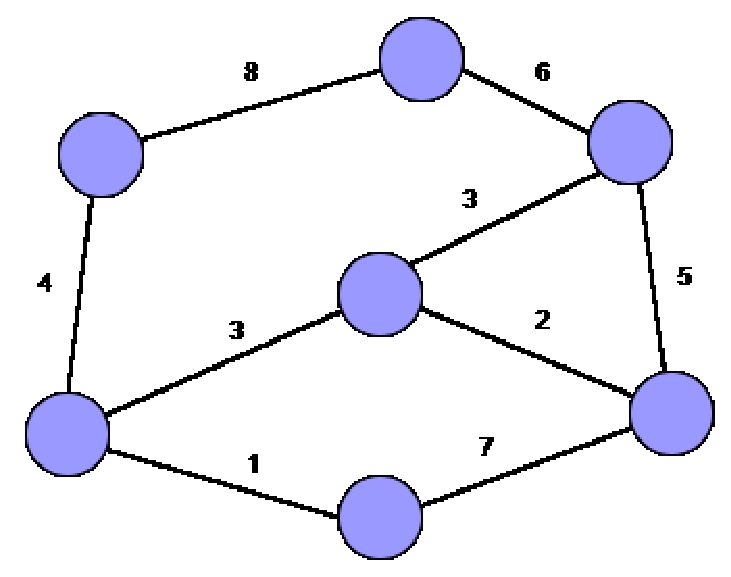
\includegraphics{images/kruskaluv_algoritmus_puvodni.eps}}\\
        \end{center}
        Vypíšeme jednotlivé ohodnocení hran a seřadíme je od nejmenších po největší:
        \begin{itemize}
            \item{4,3,1,7,2,3,5,6,8}
            \item{1,2,3,3,4,5,6,7,8}
        \end{itemize}

    \end{frame}
    
    \begin{frame}[t]
        \frametitle{Příklad Kruskalova algoritmu}
        \begin{onlyenv}<1>
            \begin{center}
                \scalebox{0.45}{\includegraphics<1>{images/kruskaluv_algoritmus_1.eps}}
            \end{center}
                \begin{itemize}
                    \item{Odstraníme všechny hrany, ale musíme si pamatovat jejich původní pozici a ohodnocení}
                \end{itemize}
        \end{onlyenv}

        \begin{onlyenv}<2>
            \begin{center}
                \scalebox{0.45}{\includegraphics<2>{images/kruskaluv_algoritmus_2.eps}}
            \end{center}
                \begin{itemize}
                    \item{Vybereme hranu s nejmenším ohodnocením (1) a přidáme ji do grafu, pokud netvoří cyklus}
                \end{itemize} 
        \end{onlyenv}

        \begin{onlyenv}<3>
            \begin{center}
                \scalebox{0.45}{\includegraphics<3>{images/kruskaluv_algoritmus_3.eps}}
            \end{center}
                \begin{itemize}
                    \item{Pokračujeme s další hranou s nejmenším ohodnocením a za stejných podmínek ji přidáme do grafu}
                \end{itemize}
        \end{onlyenv}

        \begin{onlyenv}<4>
            \begin{center}
                \scalebox{0.45}{\includegraphics<4>{images/kruskaluv_algoritmus_4.eps}}
            \end{center}
                \begin{itemize}
                    \item{Pokud máme více hran se stejným ohodnocením, můžeme si vybrat, kterou z nich přidáme}
                    \item{V tomto případě, pokud přidáme obě hrany, tak ani jedna netvoří cyklus}     
                \end{itemize} 
        \end{onlyenv}

        \begin{onlyenv}<5>
            \begin{center}
                \scalebox{0.45}{\includegraphics<5>{images/kruskaluv_algoritmus_5.eps}}
            \end{center}
                \begin{itemize}  
                    \item{Pokračujeme další hranou s nejmenším ohodnocením z hran, které jsme ještě neprošli}
                \end{itemize} 
        \end{onlyenv}

        \begin{onlyenv}<6>
            \begin{center}
                \scalebox{0.45}{\includegraphics<6>{images/kruskaluv_algoritmus_6.eps}}
            \end{center}
                \begin{itemize}
                    \item{V tomto případě nám další hrana tvoří cyklus (kružnici), do kostry ji tedy přidat nemůžeme}
                \end{itemize} 
        \end{onlyenv}

        \begin{onlyenv}<7>
            \begin{center}
                \scalebox{0.45}{\includegraphics<7>{images/kruskaluv_algoritmus_7.eps}}
            \end{center}
                \begin{itemize}
                    \item{Dle postupu pokračujeme dále a volíme další hranu, která ještě nebyla zkontrolována}
                \end{itemize}
        \end{onlyenv}

        \begin{onlyenv}<8>
            \begin{center}
                \scalebox{0.45}{\includegraphics<8>{images/kruskaluv_algoritmus_8.eps}}
            \end{center}
                \begin{itemize}
                    \item{V tomto případě hrana opět tvoří cyklus, proto ji do kostry nemůžeme použít}
                \end{itemize} 
        \end{onlyenv}

        \begin{onlyenv}<9>
            \begin{center}
                \scalebox{0.45}{\includegraphics<9>{images/kruskaluv_algoritmus_9.eps}}
            \end{center}
                \begin{itemize}
                    \item{Poslední hrana nám opět tvoří cyklus, proto ji do kostry nezahrneme}
                \end{itemize} 
        \end{onlyenv}

        \begin{onlyenv}<10>
            \begin{center}
                \scalebox{0.45}{\includegraphics<10>{images/minimalni_kostra.eps}}
            \end{center}
                \begin{itemize}
                    \item{Takto potom vypadá výsledná minimální kostra našeho grafu}         
                \end{itemize} 
        \end{onlyenv}
             
    \end{frame}

    \begin{frame}
        \frametitle{Obecný postup Kruskalova algoritmu}
        \scalebox{.9}{\begin{algorithm}[H]
            \caption{Kraskalův algoritmus}
            \KwIn{Graph *graph, Edge *edges, Vertex *vertexes}   \vspace{.25cm}
            $Graph\;min\_graph;$\hspace{2cm}$//creates\;new\;empty\;graph$ \\
            \For{all edges}{{$getweight(edge);$\hspace{2cm}$//gets\;weights\;for\;all\;edges$} \\ {$getvertexes(edge);$\hspace{1cm}$//gets\;vertexes\;for\;each\;edge$}}
            $sort(edges); \hspace{1.5cm} //sorts\;all\;weights\;from\;lowest\;to\;highest$ \\
            
            \For{all edges}{$//checks\;if\;edge\;creates\;a\;cycle,\;if\;not\;adds\;edge\;to\;min\_graph$ \\ \If{(edge != edgecycle(edge, $min\_graph$))}{$add\_edge\_to\_graph(edge, min\_graph);$}} 
            \KwRet{$min\_graph;$\hspace{1cm}$//returns\;minimal\;graph$}
        \end{algorithm}}
    \end{frame}

    \begin{frame}
        \frametitle{Časová složitost algoritmu}
        Pokud předpokládáme, že algoritmus ještě bude zjišťovat, zda-li poskytnuté vrcholy náleží danému grafu, časová složitost alogritmu bude vypadat takto: \
        \begin{center}
            $O(H\;log\;V\;+\;H \times T_{find}(V)\;+\;V \times T_{union}(V))$
        \end{center}
        Kde:
            \begin{itemize}
                \item{$T_{find}(V)$ a $T_{union}(V)$ jsou časové složitosti operací Find a Union na grafech s vrcholy V a hranami H, keré spadají do struktury Union-Find}
                \item{Union-Find je algoritmus zaměřený na zjišťování konektivity mezi jednotlivými prvky (v našem případě se jedná o zjištění cyklu mezi jednotlivými vrcholy)} 
            \end{itemize}
    \end{frame}

    \begin{frame}
        \frametitle{Časová složitost algoritmu}
        Pokud předpokládáme, že v nejhorším případě je počet vrcholů $H=V^2$ a v souladu s pravidly asymptotické složitosti můžeme dále zanedbat aditivní konstanty, dostaneme:
        \begin{center}
            $O(H \times log(H))$
        \end{center}
        Pokud jsou hrany již seřazeny nebo je možno k jejich seřazení použít řadící algoritmus s lineární složitostí (např. counting sort), tak je složitost rovna: \\
        \begin{center}
            $O(H \times \alpha (H))$
        \end{center}
        Kde:
        \begin{itemize}
            \item{$\alpha$ je inverzní Ackermanova funkce (odpovídá složitosti Union-Find)}
        \end{itemize}
    \end{frame}

    \begin{frame}
        \frametitle{Použité zdroje}
        \begin{thebibliography}{5}
            \bibitem{algoritmy} algoritmy.net
            \newblock \texttt{\href{https://www.algoritmy.net/article/1417/Kruskaluv-algoritmus}{algoritmy.net/Kruskaluv-algoritmus}}

            \bibitem{kostecky} blog.kostecky.cz
            \newblock \texttt{\href{https://blog.kostecky.cz/2016/01/kruskaluv-algoritmus-implementace-rozbor.html}{blog.kostecky.cz/Kruskaluv-algoritmus}}
            
            \bibitem{hackearth} hackearth.com
            \newblock \texttt{\href{https://www.hackerearth.com/practice/notes/disjoint-set-union-union-find/}{hackerearth.com/Find-Union}}

            \bibitem{referaty} referaty-seminarky.cz
            \newblock \texttt{\href{http://referaty-seminarky.cz/ackermannova-funkce/}{referaty-seminarky.cz/Ackermannova-funkce}}

            \bibitem{teorie} teorie-grafu.cz
            \newblock \texttt{\href{https://teorie-grafu.cz/}{teorie-grafu.cz}}
        \end{thebibliography}
    \end{frame}
\end{document}
